\documentclass[11pt]{amsart}
\usepackage{geometry}                % See geometry.pdf to learn the layout options. There are lots.
\geometry{letterpaper}                   % ... or a4paper or a5paper or ...
%\geometry{landscape}                % Activate for for rotated page geometry
%\usepackage[parfill]{parskip}    % Activate to begin paragraphs with an empty line rather than an indent
\usepackage{graphicx}
\usepackage{amssymb}
\usepackage{epstopdf}
\usepackage[usenames,dvipsnames]{color}
\usepackage{hyperref}
\usepackage{subfig}
\usepackage{float}
\usepackage{dsfont}
\usepackage{wrapfig}
\hypersetup{colorlinks=true}
\DeclareGraphicsRule{.tif}{png}{.png}{`convert #1 `dirname #1`/`basename #1 .tif`.png}
\renewcommand\familydefault{\sfdefault}
\newcommand{\todo}[1]{{\bf\textcolor{red}{TODO: #1}}}
\setlength{\topmargin}{0cm}
\setlength{\headheight}{0cm}
\setlength{\headsep}{1cm}
\setlength{\textheight}{7.7in}
\setlength{\textwidth}{6.5in}
\setlength{\oddsidemargin}{0cm}
\setlength{\evensidemargin}{0cm}
\setlength{\parindent}{0.25cm}
\setlength{\parskip}{0.1cm}

\usepackage{prettyref}
\newrefformat{sec}{Section~\ref{#1}}
\newrefformat{tbl}{Table~\ref{#1}}
\newrefformat{fig}{Figure~\ref{#1}}
\newrefformat{chp}{Chapter~\ref{#1}}
\newrefformat{eqn}{\eqref{#1}}
\newrefformat{set}{\eqref{#1}}
\newrefformat{alg}{Algorithm~\ref{#1}}
\newrefformat{apx}{Appendix~\ref{#1}}
\newcommand\pr[1]{\prettyref{#1}}

\usepackage{fancyhdr,graphicx,lastpage}% http://ctan.org/pkg/{fancyhdr,graphicx,lastpage}
\fancypagestyle{plain}{
  \fancyhf{}% Clear header/footer
  \fancyhead[L]{CSCI-GA.3033-018 - Geometric Modeling}% Right header
  \fancyhead[R]{\includegraphics[height=20pt]{nyu.pdf}}% Right header
  \fancyfoot[L]{\vspace{2pt} Daniele Panozzo}% Left footer
  \fancyfoot[R]{\vspace{2pt} \thepage}% Right footer
}
\renewcommand{\vec}[1]{\mathbf{#1}}
\newcommand{\bdm}[1]{{\begin{displaymath}#1\end{displaymath}}}
\newcommand{\mtrx}[1] {\begin{bmatrix}#1\end{bmatrix}}
\newcommand{\setR}{\mathds{R}}
\newcommand{\setC}{\mathds{C}}
\newcommand{\itemz}[1]{{\begin{itemize}{#1}\end{itemize}}}

\renewcommand{\vec}[1]{\mathbf{#1}}
\DeclareMathOperator*{\argmin}{argmin}
\def\x{\vec{x}}
\def\c{\vec{c}}
\def\p{\vec{p}}
\providecommand{\abs}[1]{\lvert#1\rvert}
\providecommand{\norm}[1]{\lVert#1\rVert}

\begin{document}

\hspace{50pt}

\begin{center}

{\huge \textbf{Assignment 4: Mesh Parametrization}}\\
\vspace{10pt}
\end{center}

In this exercise you will
\begin{itemize}
\item{Familiarize yourself with vector field design on surfaces.}
\item{Create scalar fields whose gradients align with given vector fields as closely as possible.}
\item{Experiment with the \texttt{libigl} implementation of harmonic and least-squares conformal parameterizations.}
\end{itemize}

\section{Tangent vector fields for scalar field design}
Our first task is to design smooth tangent vector fields on a surface; these
will be ``integrated'' later to define a scalar field. A (piecewise constant)
vector field on a triangle mesh is defined as an assignment of a single vector
to each triangle such that each vector lies in the tangent plane containing the
triangle. We will design fields to follow a set of alignment constraints
provided by the user: the user specifies the field vectors at a subset of the
mesh triangles (the constraints) and those constraints are interpolated smoothly
throughout the surface to define a field.

\begin{figure}[h!]
\includegraphics[width=0.5\linewidth]{vf}
\label{fig:vf}
\end{figure}

\subsection{Creating vector constraints}
The provided assignment code already implements
a minimal interface for assigning vector constraints at faces.
To use it, click on a face to select and add a constraint, and then use the "[" and "]" to adjust the constrained direction. 

\emph{Relevant} \texttt{libigl} \emph{functions: } None.
\vspace{-5mm}
\subsection{Interpolating the constraints}
Since each field vector $\vec u_f$ lies in the plane of its respective triangle
$f$, it can be decomposed into the triangle's local basis and represented with
two real coefficients: $\vec u_f = (x_f, y_f) \in \setR^2$. Alternatively, we can
identify the triangle plane with the complex plane, expressing the vector as a
single complex number $u_f = x_f + i y_f \in \setC$. 

The interpolation produces a smooth vector field from the constraints by trying
to make each vector as similar as possible to the adjacent triangles' vectors.
However, since vectors $u_f$, $u_g$ at adjacent triangles $f$, $g$
are expressed with respect to the triangles' local bases, and the
triangles generally have different bases,
their complex expressions cannot be compared directly (see inset figure). So we
must first express the vectors with respect to a common basis.

A simple way to choose a common basis is to use the shared (directed) edge
vector as the new real ($x$) axis for both triangles. This implicitly also chooses the
$90^\circ$-counterclockwise-rotated edge vector as the imaginary axis, forming
a complete basis. In this new common basis, the two triangles' vectors can be
written as $\tilde u_f = u_f e_f^{-1} = u_f \overline{e_f}$, $\tilde u_g = u_g
\overline{e_g}$. Where $e_f$, $e_g$ are the shared edge vector expressed in
each local basis. Here $\overline{e_f}$ denotes the complex conjugate of $e_f$,
\emph{and we assume $e_f$, $e_g$ are normalized so that the conjugate is
actually the inverse}---normalize them!

\begin{wrapfigure}{l}{0.4\columnwidth}
  \vspace{-20pt}
    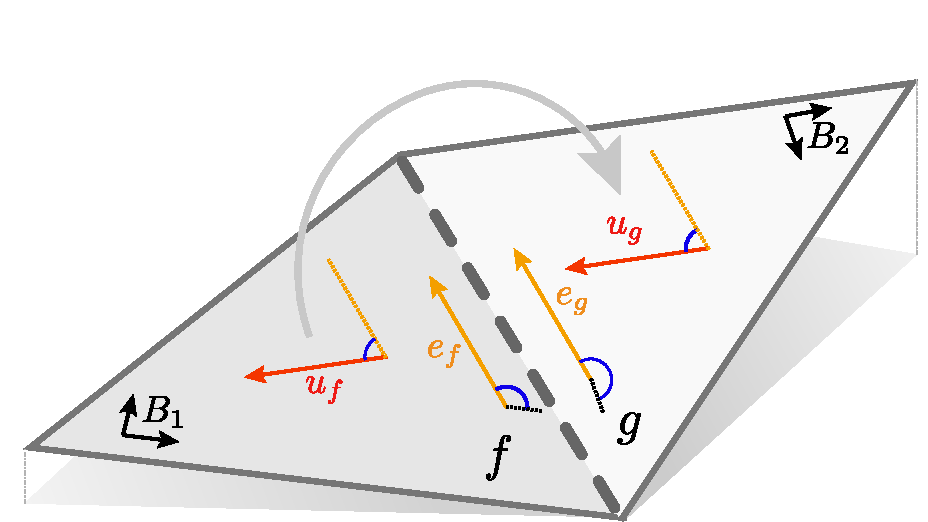
\includegraphics[width=.4\columnwidth]{2.pdf}
  \vspace{-20pt}
\end{wrapfigure}
The difference (``non-smoothness'') of the two vectors across the edge  $(f,g)$
can now be computed as $E_{fg}(u_f, u_g) = \| u_f \overline{e_f} - u_g \overline{ e_g}\|^2$
(recall that $\|z\|^2 = z \overline{z}$ is a complex number $z$'s squared magnitude).
This is a quadratic form on the complex variables $u_f$, $u_g$ and can be
manipulated into the form $E_{fg}(u_f, u_g) =
\mtrx{\overline{u_f}&\overline{u_g}}  Q_{fg} \mtrx {u_f\\u_g}$ for a particular
complex matrix $Q_{fg}$. The full field's smoothness can then be written as the
sum of all these per-edge energies: $\sum_{\textrm{edge}(f,g) }
E_{fg}(u_f, u_g)$. This yields a sparse quadratic form $u^* Q u$, where the
complex column vector $u$ encodes each each per-face vector. The row
vector $u^*$ is $u$'s adjoint (conjugate transpose), and $Q$ is the
appropriate combination of the matrices $Q_{fg}$. Thus, finding the smoothest
field under the prescribed constraints is equivalent solving
\begin{eqnarray*}
&&\min ~~u^* Q u\\
&\textrm{such that}&~~ u|_{cf} = c,
\end{eqnarray*}
where $cf$ are the constrained face indices and $c$ are the prescribed vectors
at those faces. We can differentiate the smoothness energy to find its minimum,
thus obtaining a (complex) linear system
\begin{align*}
    Q u &= 0 \\
    \textrm{such that}~~ u|_{cf} &= c.
\end{align*}
This system's solution describes the smoothly interpolated vector field
(Fig.~\ref{fig:vf_interp}). Your task is 
\itemz{
\item Determine how to construct the complex matrix Q,
\item Solve the system under the prescribed constraints (which are specified via the UI as described above),
\item Display the constraints and the interpolated field when '2' is pressed.
}
\emph{Note:} Eigen supports sparse complex matrices and can factorize/solve
linear systems with them (e.g. \texttt{SparseLU}), but feel free to convert
this problem into real variables if you find that easier.

\emph{Relevant} \texttt{libigl} \emph{functions: }
\texttt{igl::sparse},\texttt{igl::colon},\texttt{ igl::slice},\texttt{
    igl::slice\_into},\texttt{ igl::cat}, \texttt{igl::kronecker\_product},
\texttt{igl::speye}, \texttt{igl::repdiag} can be used for various sparse matrix
construction and manipulation operations. \texttt{igl::local\_basis} computes
a basis for each triangle plane.

Required output for this section:
\itemz{
\item{Visualization of the constraints and interpolated field.}
\item{An ASCII dump of the interpolated field ($\#F \times 3$ matrix, one
    vector per row) for the mesh \texttt{irr4-cyl2.off} and the input
    constraints in the provided file \texttt{irr4-cyl2.constraints}.}
}

\section{Reconstructing a scalar field from a vector field}
Your task is now to find a scalar function $S(\x)$ defined over the surface
whose gradient fits a given vector field as closely as possible.
The scalar field is defined by values on the mesh vertices that are
linearly interpolated over each triangle's interior: for given vertex values
$s_i$, the function $S(\x)$ inside a triangle $t$ is computed as $S_t(\x) =
\sum\limits_{\textrm{vertex}~i~\in~t}^3 s_i \phi_i^t(\x)$, where $\phi_i^t(\x)$ are the
linear ``hat'' functions associated with each triangle vertex (i.e. $\phi_i^t(\x)$
is linear and takes the value $1$ at vertex $i$ and $0$ at all other vertices).
Then the scalar function's (vector-valued) gradient is $\vec g_t = \nabla
S_t = \sum\limits_{\textrm{vertex}~i~\in~t}^3 s_i \nabla\phi_i^t$. 

Since the ``hat'' functions are piecewise linear, their  gradients
$\nabla\phi_i^t$ are constant within each triangle, and so is $\vec g_t$ (the
full scalar function's gradient). Specifically, $\vec g_t$ is a
linear combination of the constant hat function gradients with the (unknown)
values $s_i$ as coefficients, meaning that we can write an expression of the
form $g  = G s$, where $s$ is a $\#V\times 1$ column vector holding each
$s_i$, $g$ is a column vector of size $3\#F\times 1$
consisting of the vectors $\vec g_t$ ``flattened'' and vertically stacked, and
$G$ is the so-called ``gradient matrix'' of size $3\#F\times \#V$.

Since there is no guarantee that our interpolated face-based field is actually
the gradient of some function, we cannot attempt to integrate it directly.
Instead, we will try to find $S(\x)$ by asking its gradient to approximate the
vector field $u$ in the least-squares sense:
\bdm{
\min ~~\sum\limits_{\textrm{face}~t} A_t \|\vec g_t-\vec u_t\|^2,\\
}
where $A_t$ is triangle $t$'s area, $\vec g_t$ is the (unknown) function
gradient on the triangle, and $\vec u_t$ is the triangle's vector assigned by
the guiding vector field. Using the linear relationship $g = Gs$, we can write
this least-squares error as a (real) quadratic form:
$$s^TKs + s^Tb + c$$
and minimize it by solving a linear system for the unknown $s$.

\itemz{
    \item Determine the matrix $K$ and vector $b$ in the above minimization (by
        expanding the least-squares error expression).
\item Minimize by differentiating and equating the gradient to zero; this gives
    you a linear system to solve.
\item Display the scalar function on the surface using a color map and overlay
    its gradient vectors when the user presses '3'.
\item Plot the deviation between the input vector field and the solution scalar
    function's gradient (the ``Poisson reconstruction error'').
}

\emph{Note:}
the linear system is not full rank; $K$ has a one dimensional nullspace
corresponding to the constant function. This is because a scalar field can be
offset by any constant value without altering its gradient. You will need to
fix the value at one vertex (e.g., to zero) to solve the system.

\begin{figure}[h!]
   \centering
   \subfloat[Vector Field]{\label{fig:sf_vf}\includegraphics[width=0.23\linewidth]{sf_vf}} 
\hspace{2cm}
   \subfloat[Scalar Field]{\label{fig:sf_sg}\includegraphics[width=0.23\linewidth]{sf_sg.png}} 
   \caption{A vector field and the reconstructed scalar function. Note the
    scalar function gradient's deviation from the input field.}
   \label{fig:vf}
\end{figure}

\emph{Relevant} \texttt{libigl} \emph{functions: } \texttt{igl::grad}
calculates the gradient matrix explained above. \texttt{igl::doublearea} can be
used to compute triangle areas. \texttt{igl::sparse},
\texttt{igl::repdiag}, \texttt{igl::colon}, \texttt{igl::slice},
\texttt{igl::slice\_into} might also be relevant here.

Required output for this section:
\itemz{
\item{Visualization of computed scalar function and its gradient.}
\item{Plots of the Poisson reconstruction error}
\item{An ASCII dump of the reconstructed scalar function ($\#V \times 1$ vector,
    one vertex value per row) for the mesh \texttt{irr4-cyl2.off} and the input
    constraints in \texttt{irr4-cyl2.constraints}. }
}

\section{Harmonic and LSCM Parameterizations}
For this task, you will experiment with flattening a mesh with a boundary onto
the plane using two parameterization methods: \emph{harmonic} and \emph{Least
Squares Conformal} (LSCM) parameterization. In both cases, two scalar fields,
$U$ and $V$, are computed over the mesh. The per-vertex ($u$, $v$) scalars
defining these coordinate functions determine the vertices' flattened positions
in the plane (the flattening is linearly interpolated within each triangle). 

For the harmonic parametrization example, you will first map the mesh boundary
to a unit circle in the UV plane centered at the origin. The boundary $U$ and
$V$ coordinates are then ``harmonically interpolated'' into the interior by
solving the Laplace equation with Dirichlet boundary conditions (setting the
Laplacian of $U$ equal to zero at each interior vertex, then doing the same for
$V$). This involves two separate linear system solves (each with the same
system matrix).

In LSCM, the boundary is free, with the exception of two vertices that must be
fixed at two different locations in the UV-plane (to pin down a global
position, rotation, and scaling factor). These vertices can be chosen
arbitrarily. The process is again a linear system solve, but in this case the
$U$ and $V$ functions are entwined into a single linear system.

\itemz{
\item Use the \texttt{libigl} implementation of harmonic (key '4') and
    LSCM (key '5') mappings. Hitting these keys should trigger a visualization
    of one of the two mapping functions ($U$ or $V$) as a color map over the
    surface, with the provided line texture overlaid.
\item Compute the gradient of the selected mapping function and overlay it (key '6').
}

\begin{figure}[h!]
   \centering
   \subfloat[Harmonic]{\label{fig:harmonic}\includegraphics[width=0.23\linewidth]{harmonic}} 
%\hspace{.2cm}
   \subfloat[Gradient of V]{\label{fig:harmonic_grad}\includegraphics[width=0.23\linewidth]{harmonic_grad}} 
%\hspace{.2cm}
   \subfloat[UV]{\label{fig:harmonic_uv}\includegraphics[width=0.14\linewidth]{harmonic_uv}} 
%\hspace{.2cm}
   \subfloat[LSCM]{\label{fig:lscm}\includegraphics[width=0.23\linewidth]{lscm}} 
%\hspace{.2cm}
   \subfloat[UV]{\label{fig:lscm_uv}\includegraphics[width=0.14\linewidth]{lscm_uv}} 
%\hspace{.2cm}
   \caption{A harmonic parameterization (A), the gradient of its $V$ function
    (B) and a visualization of the flattened mesh on the $UV$ plane (C). LSCM
    parameterization (D) and its $UV$ domain (E).} \label{fig:harmonic_lscm}
\end{figure}

\emph{Note:} you may need to scale up the parameterization to better visualize
the texture lines (parametric curves).

\emph{Relevant} \texttt{libigl} \emph{functions: } \texttt{igl::harmonic},
\texttt{igl::lscm}, \texttt{igl::boundary\_loop},
\\\texttt{igl::map\_vertices\_to\_circle}.


Required output for this section:
\itemz{
\item{Visualization of the computed mapping functions and their gradients for
    LSCM and harmonic mapping.}
}
\vspace{-5mm}
\section{Editing a parameterization with vector fields}
A parameterization consists of two scalar coordinate functions on the surface.
As such, we can use vector fields to guide the parameterization: we can design
a vector field and fit one of the coordinate functions' gradients to it.

\subsection {Editing the parameterization}
Starting with a harmonic/LSCM parameterization, use the results of the previous
steps to replace one of the $U$, $V$ functions with a function obtained from a
smooth user-guided vector field. Visualize the resulting $U$ or $V$ replacement
function and its gradient atop the mesh, and texture the mesh with the new
parameterization (key '7').

\begin{figure}[h!]
   \centering
   \subfloat[Harmonic]{\label{fig:paramedit_harmonic}\includegraphics[width=0.22\linewidth]{paramedit_harmonic}} 
\hspace{.2cm}
   \subfloat[Constraints]{\label{fig:paramedit_constraints}\includegraphics[width=0.22\linewidth]{paramedit_constraints}} 
\hspace{.2cm}
   \subfloat[Vector Field]{\label{fig:paramedit_vf}\includegraphics[width=0.22\linewidth]{paramedit_vf}} 
\hspace{.2cm}
   \subfloat[Parameterization]{\label{fig:paramedit_edited}\includegraphics[width=0.22\linewidth]{paramedit_edited}} 
   \caption{An initial harmonic parameterization (A) is edited by designing a
    vector field. The user-provided constraints (B) are first interpolated (C),
    then a scalar function is reconstructed and used to replace the
    parameterization's $V$ coordinate function. The new scalar function and its
    gradient are shown in (D) together with the newly textured mesh.\vspace{-5mm}}
   \label{fig:paramedit}
\end{figure}

\subsection {Detecting problems with the parameterization}
It is possible for a parameterization created in this way to cause triangles to
flip over as they are mapped into the $UV$ plane. Determine a reliable
criterion for detecting flipped triangles and visualize the planar mapped mesh
with the flipped faces highlighted in red (key '8'). 

Required output for this section:
\itemz{
\item{Visualization of the edited parameterization.}
\item{Visualization of flipped elements.}
\item{An ASCII dump of the flipped triangle indices (if any) resulting from an
    edited harmonic parameterization of the mesh \texttt{irr4-cyl2.off}, where
    the parameterization's $V$ coordinate is replaced with a scalar field
    designed from the gradient vector constraints provided in
    \texttt{irr4-cyl2.constraints}.}
}

\end{document}  
